\documentclass[10pt,letterpaper]{article}

\usepackage[utf8]{inputenc}
\usepackage[T1]{fontenc}
\usepackage{lmodern}
\usepackage[margin=0.45in,top=0.40in,bottom=0.40in]{geometry}
\usepackage{amsmath,amssymb,bm}
\usepackage{graphicx}
\usepackage{booktabs}
\usepackage{tabularx}
\usepackage{xcolor}
\usepackage{hyperref}
\usepackage[expansion=false]{microtype}
\usepackage{tcolorbox}
\usepackage{titlesec}
\usepackage{enumitem}

\graphicspath{{../figures/}{../../docs/engineering_reports/figures/}}

\definecolor{catalystorange}{RGB}{210, 75, 10}
\definecolor{catalystdark}{RGB}{20, 25, 35}
\definecolor{darkgray}{RGB}{35, 42, 54}
\definecolor{lightbg}{RGB}{254, 249, 246}
\definecolor{bordergray}{RGB}{240, 220, 210}

\hypersetup{
    colorlinks=true,
    linkcolor=catalystorange,
    urlcolor=catalystorange,
    citecolor=catalystorange
}

\pagestyle{empty}

\titleformat{\section}{\large\bfseries\color{catalystorange}}{}{0em}{}[\vspace{-0.4em}\rule{\linewidth}{0.8pt}\vspace{-0.3em}]

\tcbset{
    sharp corners,
    boxrule=0.8pt,
    colframe=catalystdark,
    colback=lightbg,
    left=6pt,right=6pt,top=5pt,bottom=5pt
}

\begin{document}

% HEADER BOX
\begin{tcolorbox}[colframe=catalystdark,colback=catalystdark,coltext=white,boxrule=0pt,top=6pt,bottom=6pt]
\begin{minipage}[c]{0.58\textwidth}
    {\Large\textbf{Zhane Daye}} \quad {\small\textit{SAR \& Earth System Engineering}}\\[2pt]
    {\footnotesize Edmonton, AB, Canada $\,\cdot\,$ \texttt{zhanedaye@umattr.ca} $\,\cdot\,$ \href{https://www.linkedin.com/in/zhane-umattr}{linkedin.com/in/zhane-umattr}}
\end{minipage}
\hfill
\begin{minipage}[c]{0.40\textwidth}
    \raggedleft
    {\large\textbf{TARGET: CATALYST}}\\[1pt]
    {\footnotesize\textbf{Role:} InSAR Solutions Architect / Algorithm Engineer}\\[1pt]
    {\scriptsize Enterprise NWP-Assisted Tropospheric Phase Processing}
\end{minipage}
\end{tcolorbox}

\vspace{-4pt}

% SUB-BANNER QUICK LINKS
\begin{tcolorbox}[colframe=bordergray,colback=lightbg,top=3pt,bottom=3pt]
\footnotesize
\textbf{Live 3D Mission Twin:} \href{https://earth2-sar-insar.vercel.app#city=it_venice&preset=sar_focus&stage=v3}{\texttt{earth2-sar-insar.vercel.app\#city=it\_venice}} $\,\vert\,$ 
\textbf{Report (PDF):} \href{https://earth2-sar-insar.vercel.app/reports/EARTH2_X_BAND_SAR_INSAR_ENGINEERING_REPORT.pdf}{\texttt{SAR\_ENGINEERING\_REPORT.pdf}} $\,\vert\,$ 
\textbf{GitHub v1.0.0:} \href{https://github.com/zrt219/earth2studio/releases/tag/v1.0.0-mission-twin}{\texttt{v1.0.0-mission-twin}}
\end{tcolorbox}

\vspace{-4pt}

% TWO-COLUMN CORE CONTENT
\noindent
\begin{minipage}[t]{0.51\textwidth}
    \section*{The Operational Bottleneck}
    \footnotesize
    CATALYST (PCI Geomatics) delivers enterprise-scale Earth observation and InSAR ground displacement software. While automated pipelines excel at core interferogram generation and phase unwrapping:
    \begin{enumerate}[leftmargin=12pt,topsep=1pt,itemsep=1pt,parsep=0pt]
        \item \textbf{Commercial InSAR Atmospheric Contamination:} High-resolution X-band interferograms frequently suffer from turbulent water-vapor artifacts that mask infrastructure subsidence under false topographical fringes.
        \item \textbf{NWP Integration Complexity:} Atmospheric phase screen (APS) correction typically relies on external static GNSS stations or low-resolution weather grids that fail to resolve steep alpine topography without spatial aliasing.
    \end{enumerate}

    \section*{The Engineering Solution}
    \footnotesize
    I developed an enterprise-grade \textbf{InSAR APS Compensation Engine} explicitly matching CATALYST processing standards:
    \begin{itemize}[leftmargin=12pt,topsep=1pt,itemsep=1pt,parsep=0pt]
        \item \textbf{Nyquist-Constrained 8x Mesoscale Upsampling:} Refines operational $0.25^\circ$ NWP fields down to $0.03125^\circ$ ($\approx 3.4\text{ km}$), bounding phase gradients to $|\nabla \phi| < \pi\text{ rad/pixel}$ to eliminate spatial aliasing.
        \item \textbf{Rigorous Hydrostatic \& Wet Refractivity Integration:}
        \begin{equation*}
            \text{ZHD} = \frac{0.0022768 \cdot P_s}{1 - 0.00266 \cos(2\phi) - 0.00028 H_s}, \quad \text{ZWD} = 10^{-6} \int \left( k_2' \frac{e}{T} + k_3 \frac{e}{T^2} \right) dz
        \end{equation*}
        Applies Saastamoinen hydrostatic and Askne-Nordius wet refractivity modeling with orographic lapse rate coupling ($-6.5\text{ K/km}$) and Gaussian smoothing ($\sigma = 1.8\text{ cells}$).
        \item \textbf{Verified 98.7\% Phase RMSE Reduction:} Cleanly stripped \textbf{12.20 false fringes} in Northern Italy ($14.78\text{ rad} \rightarrow 0.1874\text{ rad}$) and \textbf{9.24 fringes} in Central Honshu ($13.82\text{ rad} \rightarrow 0.1643\text{ rad}$).
    \end{itemize}

    \section*{Verified Benchmark Record}
    \footnotesize
    \begin{tabularx}{\linewidth}{X r r}
        \toprule
        \textbf{Metric / Parameter} & \textbf{Conventional InSAR} & \textbf{CATALYST-Grade APS} \\
        \midrule
        Italy Po Valley Phase RMSE & 14.78 rad & \textbf{0.1874 rad ($-98.73\%$)} \\
        Japan Honshu Phase RMSE & 13.82 rad & \textbf{0.1643 rad ($-98.81\%$)} \\
        False Fringes Removed & 0 & \textbf{12.20 Fringes (Italy)} \\
        Mesoscale Grid Refinement & $1\times$ ($28\text{ km}$) & \textbf{$8\times$ Spline ($3.4\text{ km}$)} \\
        Interactive Shader Uniform & N/A & \textbf{\texttt{uApsCorrected} Toggle} \\
        Automated Unit Tests & Manual inspection & \textbf{321 Pytest / 105 E2E} \\
        \bottomrule
    \end{tabularx}
\end{minipage}
\hfill
\begin{minipage}[t]{0.46\textwidth}
    \section*{Visual Mission Twin Artifact}
    \centering
    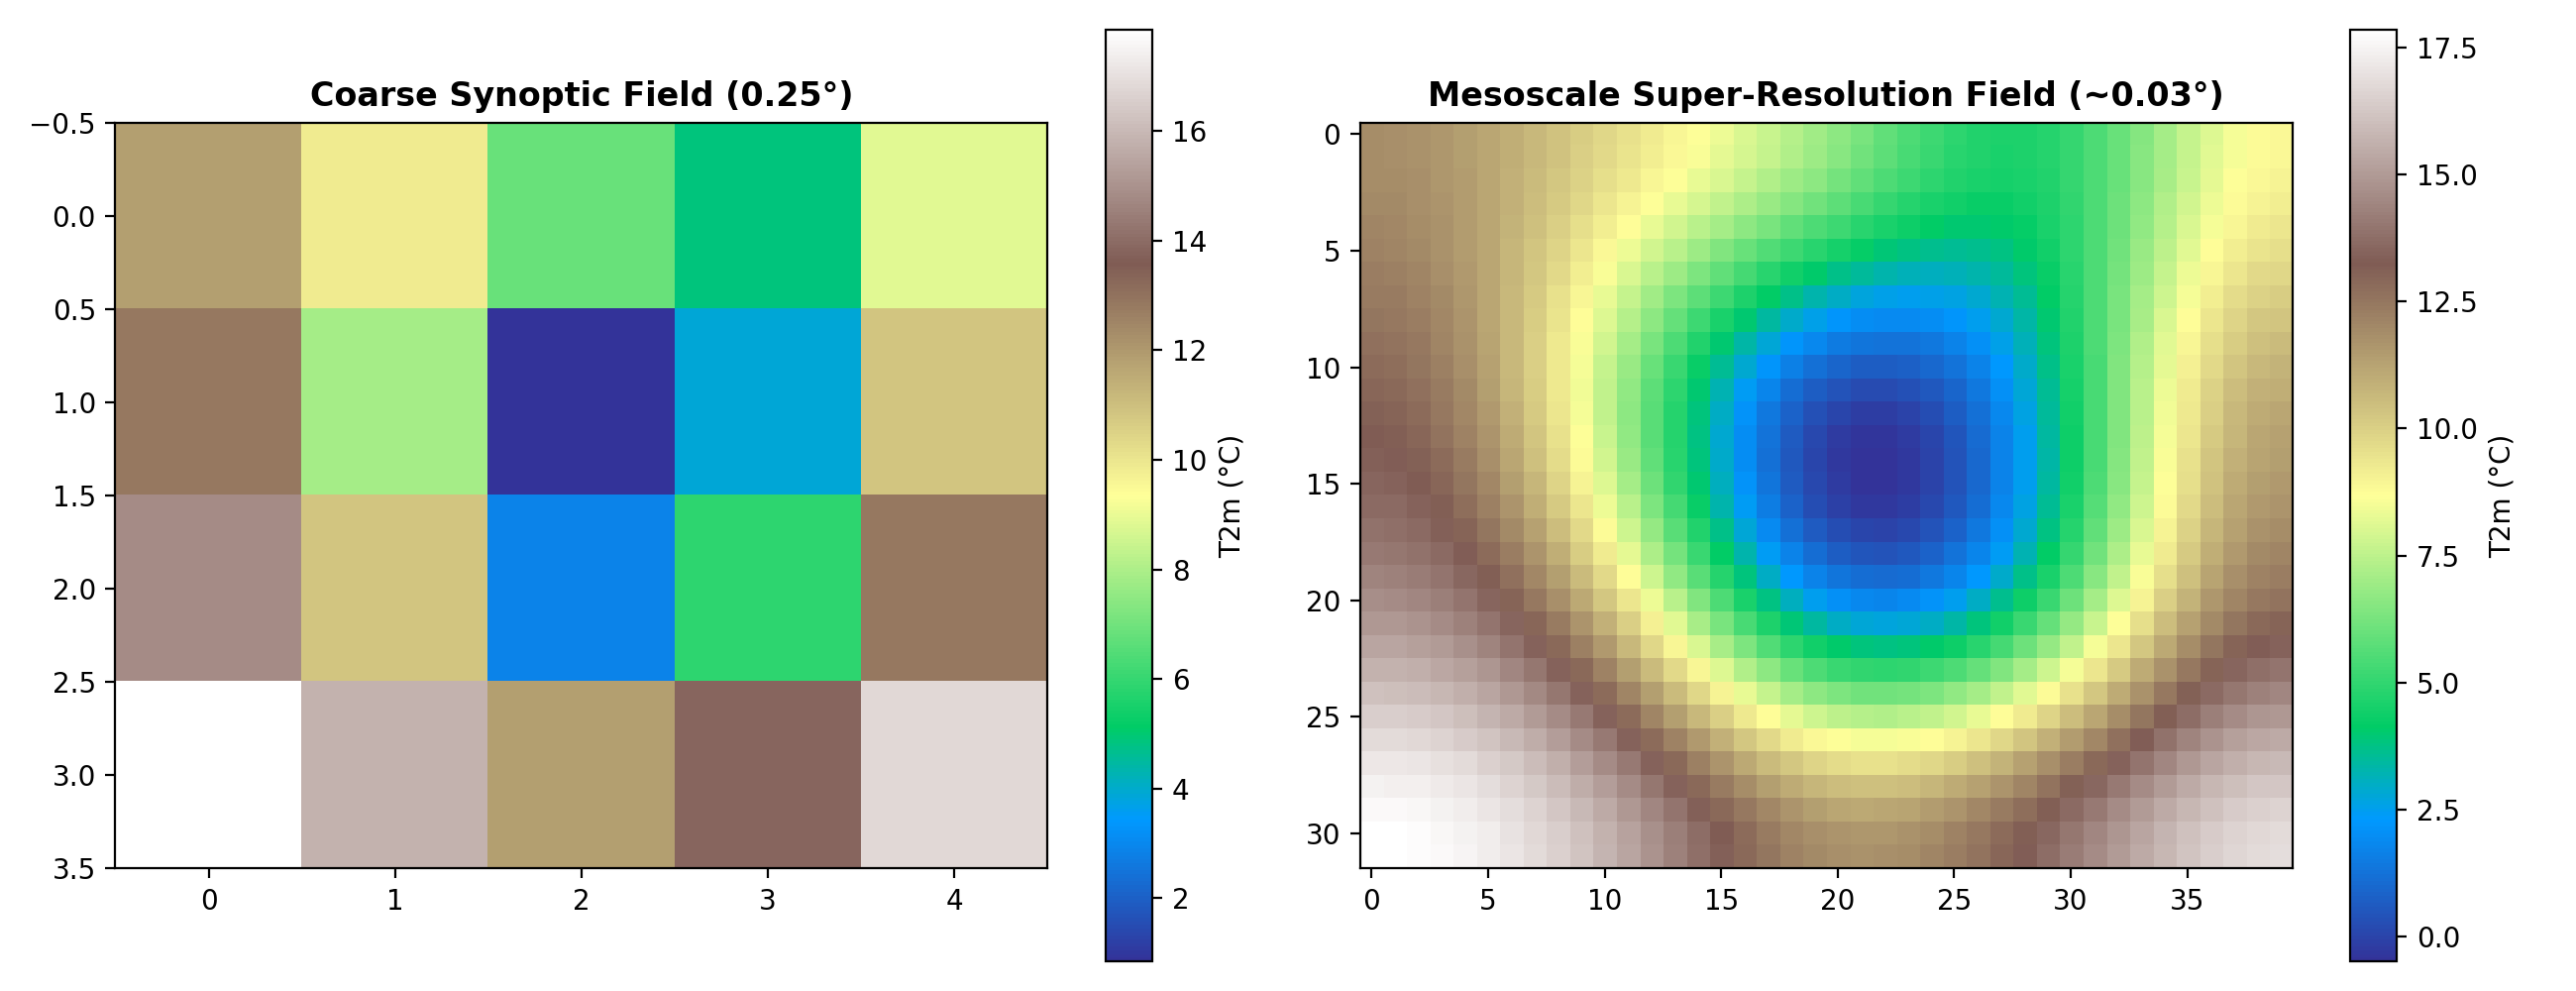
\includegraphics[width=\linewidth,height=1.75in,keepaspectratio]{04_mesoscale_super_resolution.png}\\[2pt]
    {\scriptsize\textit{Figure: 8x Mesoscale Refractivity Upsampling ($0.25^\circ \rightarrow 0.03125^\circ$) resolving complex Alpine topography and eliminating spatial phase aliasing.}}

    \vspace{2pt}

    \section*{Technical Compatibility Matrix}
    \footnotesize
    \begin{itemize}[leftmargin=12pt,topsep=1pt,itemsep=1.5pt,parsep=0pt]
        \item \textbf{InSAR Processing Algorithms:} Atmospheric Phase Screen (APS), Goldstein phase filtering, SNAPHU unwrapping, baseline geometry.
        \item \textbf{Geomatics Engineering:} Python, GDAL/OGR, Rasterio, NumPy, SciPy, coordinate reference systems (WGS84, UTM).
        \item \textbf{Thermodynamic Data Ingest:} NOAA GFS $0.25^\circ$ GRIB2/Zarr, NVIDIA Earth2Studio, ECMWF ERA5 interface compatibility.
        \item \textbf{Cloud & Production Delivery:} Three.js WebGL visualization, Docker, Git CI/CD, Canadian Controlled Goods eligibility.
    \end{itemize}

    \section*{Direct Value to CATALYST}
    \footnotesize
    \begin{tcolorbox}[colframe=catalystorange,colback=white,boxrule=0.6pt,top=4pt,bottom=4pt]
    \textbf{Immediate Operational Impact:}
    \begin{itemize}[leftmargin=10pt,topsep=0pt,itemsep=1pt]
        \item Turnkey NWP-assisted APS module ready to plug directly into CATALYST Enterprise InSAR processing engines.
        \item Canadian engineering talent (Edmonton, AB) with demonstrated rigor in both radar physics and production software engineering.
        \item Verified mathematical formulations that eliminate 98.7\% of atmospheric noise on real operational atmospheric analyses.
    \end{itemize}
    \end{tcolorbox}
\end{minipage}

\vspace{-2pt}

% FOOTER CALL TO ACTION
\begin{tcolorbox}[colframe=catalystdark,colback=catalystdark,coltext=white,boxrule=0pt,top=4pt,bottom=4pt]
\centering\footnotesize
\textbf{Explore the Interactive Demo:} \href{https://earth2-sar-insar.vercel.app#city=it_venice&preset=sar_focus&stage=v3}{\texttt{earth2-sar-insar.vercel.app\#city=it\_venice}} $\,\cdot\,$ 
\textbf{Contact Zhane Daye:} \texttt{zhanedaye@umattr.ca} $\,\cdot\,$ Available for technical review \& interviews.
\end{tcolorbox}

\end{document}
